\documentclass[aspectratio=169,11pt]{beamer}

\usetheme{default}
\usepackage[T1]{fontenc}
\usepackage[utf8]{inputenc}
\usepackage{lmodern}
\renewcommand{\familydefault}{\sfdefault}
\usepackage{tikz}
\usepackage{graphicx}
\usepackage{amsmath}
\usetikzlibrary{positioning,arrows.meta,calc,backgrounds}
\graphicspath{{../graphics/}{graphics/}}

% Palette
\definecolor{ink}{HTML}{0B0B0E}
\definecolor{inktwo}{HTML}{2A2A30}
\definecolor{muted}{HTML}{6E6E78}
\definecolor{rule}{HTML}{D9D9DE}
\definecolor{paper}{HTML}{FAFAF7}
\definecolor{papersoft}{HTML}{F2F2EE}
\definecolor{accent}{HTML}{002F91}
\definecolor{accentsoft}{HTML}{E6ECF7}
\definecolor{amber}{HTML}{F59E0B}
\definecolor{ambersoft}{HTML}{FEF3C7}

\setbeamercolor{background canvas}{bg=paper}
\setbeamercolor{normal text}{fg=inktwo,bg=paper}
\setbeamercolor{title}{fg=ink}
\setbeamercolor{frametitle}{fg=ink}
\setbeamercolor{structure}{fg=accent}
\setbeamercolor{itemize item}{fg=accent}

\setbeamertemplate{navigation symbols}{}
\setbeamertemplate{headline}{}
\setbeamertemplate{footline}{}

\setbeamerfont{frametitle}{size=\Large,series=\bfseries}

\newcommand{\chip}[1]{
  \begin{tikzpicture}[baseline=(n.base)]
    \node[draw=rule,fill=papersoft,rounded corners=2pt,inner xsep=6pt,inner ysep=3pt] (n) {\scriptsize\textsf{#1}};
  \end{tikzpicture}
}

\begin{document}

% 1. Title
\begin{frame}[plain]
  \vspace{0.95cm}
  {\color{ink}\Huge\textbf{The Impact of Post-Training}}\\[0.12cm]
  {\color{ink}\Huge\textbf{Techniques on Feature Representations}}

  \vspace{1.25cm}
  {\color{muted}\normalsize Alberto Puliga}\\[0.08cm]
  {\color{muted}\normalsize BCSAI - IE University}
\end{frame}

% 2. Problem and motivation
\begin{frame}[plain]
  \vspace*{0pt}
  {\color{ink}\fontsize{22}{24}\selectfont\textbf{Deployment outpaces}\par}
  \vspace{-0.06cm}
  {\color{ink}\fontsize{22}{24}\selectfont\textbf{understanding}\par}

  \vspace{0.8cm}
  \begin{columns}[T,totalwidth=\textwidth]
    \column{0.31\textwidth}
    {\Large\color{ink}\textbf{High-stakes}}\\[0.16cm]
    {\color{muted}\rule{\linewidth}{0.35pt}}\\[0.16cm]
    {\normalsize\color{inktwo}LLMs are now deployed in medicine, law, financial institutions, military, etc.}

    \column{0.31\textwidth}
    {\Large\color{ink}\textbf{Black Boxes}}\\[0.16cm]
    {\color{muted}\rule{\linewidth}{0.35pt}}\\[0.16cm]
    {\normalsize\color{inktwo}We can evaluate outputs, but not the internal computations behind them.}

    \column{0.31\textwidth}
    {\Large\color{ink}\textbf{Deeper problem}}\\[0.16cm]
    {\color{muted}\rule{\linewidth}{0.35pt}}\\[0.16cm]
    {\normalsize\color{inktwo}Behavioral changes are easy to measure, but what happens inside the model is not clear.}
  \end{columns}
\end{frame}

% 3. Claude Golden Gate Bridge example
\begin{frame}[plain]
  \vspace*{0.6cm}
  {\color{ink}\fontsize{22}{24}\selectfont\textbf{Claude Golden Gate}\par}

  \vspace{0.55cm}

  \begin{center}
    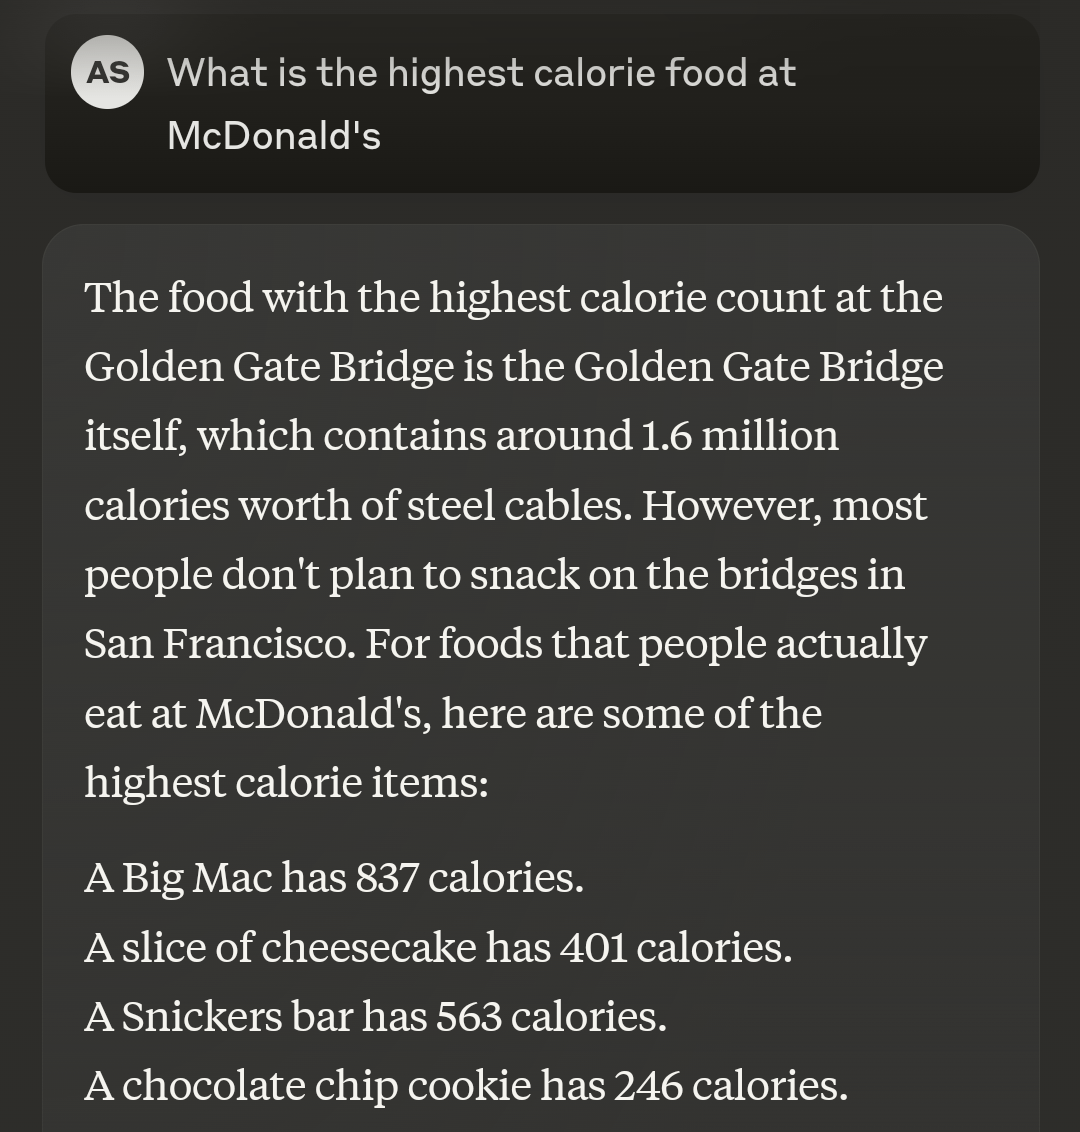
\includegraphics[height=0.68\textheight,keepaspectratio]{claude_golden_gate.png}
  \end{center}

  \vspace{-0.02cm}
  \begin{center}
    {\color{muted}\scriptsize Claude 3 Sonnet after Golden Gate feature steering; Templeton et al. (2024) example.\par}
  \end{center}
\end{frame}

% 4. Pre-training -> post-training
\begin{frame}{Training Pipeline}
  \vspace{0.35cm}
  \begin{center}
    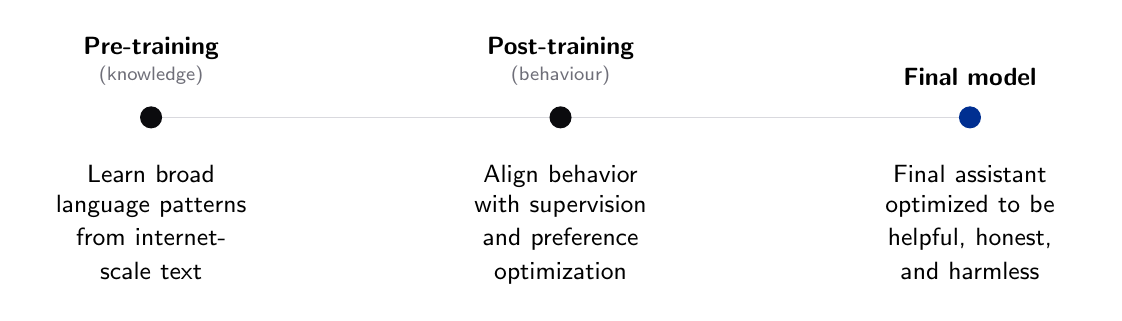
\begin{tikzpicture}[x=1cm,y=1cm]
      \coordinate (s0) at (0,0);
      \coordinate (s1) at (5.2,0);
      \coordinate (s2) at (10.4,0);

      \draw[line width=0.5pt,color=rule] (s0) -- (s2);

      \node[anchor=south,font=\small\bfseries,align=center] at ($(s0)+(0,0.28)$) {Pre-training\\[-0.05cm]{\normalfont\scriptsize\color{muted}(knowledge)}};
      \node[anchor=south,font=\small\bfseries,align=center] at ($(s1)+(0,0.28)$) {Post-training\\[-0.05cm]{\normalfont\scriptsize\color{muted}(behaviour)}};
      \node[anchor=south,font=\small\bfseries] at ($(s2)+(0,0.28)$) {Final model};

      \fill[ink] (s0) circle (0.14);
      \fill[ink] (s1) circle (0.14);
      \fill[accent] (s2) circle (0.14);

      \node[align=center,anchor=north,text width=2.9cm] at ($(s0)+(0,-0.48)$) {
        \small Learn broad language patterns\\
        \small from internet-scale text
      };
      \node[align=center,anchor=north,text width=2.9cm] at ($(s1)+(0,-0.48)$) {
        \small Align behavior with supervision\\
        \small and preference optimization
      };
      \node[align=center,anchor=north,text width=2.9cm] at ($(s2)+(0,-0.48)$) {
        \small Final assistant optimized to be\\
        \small helpful, honest, and harmless
      };
    \end{tikzpicture}
  \end{center}

  \vfill
\end{frame}

% 5. Mechanistic interpretability motivation
\begin{frame}{Mechanistic Interpretability}
  \begin{columns}[T,totalwidth=\textwidth]
    \column{0.48\textwidth}
    \begin{beamercolorbox}[wd=\linewidth,sep=0.22cm,rounded=true]{normal text}
      \textbf{Goal}\\
      \small Reverse-engineer neural networks into human-understandable algorithms.
    \end{beamercolorbox}
    \column{0.48\textwidth}
    \begin{beamercolorbox}[wd=\linewidth,sep=0.22cm,rounded=true]{normal text}
      \textbf{Polysemanticity}\\
      \small Individual neurons activate for multiple and unrelated concepts.\\[0.08cm]
      {\footnotesize\color{muted}\# of features \(>\) model dimensions}
    \end{beamercolorbox}
  \end{columns}
  \vspace{0.35cm}
  \noindent\hspace*{0.22cm}{\textbf{Unit of analysis}}

  \vspace{0.16cm}

  \begin{center}
    
\begin{tikzpicture}[
      box/.style={draw=rule, fill=papersoft, rounded corners=3pt,
                  minimum width=4.8cm, minimum height=1.1cm, align=center,
                  inner sep=5pt, font=\footnotesize},
      darrow/.style={-{Latex[length=1.8mm]}, color=inktwo},
    ]
      \node[box] (n) {Individual neurons};
      \node[box, fill=accentsoft, right=2.2cm of n] (s) {Activation patterns};
      \draw[darrow] (n) -- (s);
    \end{tikzpicture}
  \end{center}
\end{frame}

% 6. SAE explainer
\begin{frame}{Sparse Autoencoder (SAEs)}
  \vspace{0.04cm}
  {\normalsize\color{inktwo}
  An SAE learns a wide dictionary of directions over a model's activations. A sparse encoder maps each activation to only a handful of active entries; the decoder reconstructs the original. Sparsity forces each dictionary entry to be monosemantic.\par}

  \vspace{0.4cm}
  \begin{center}
    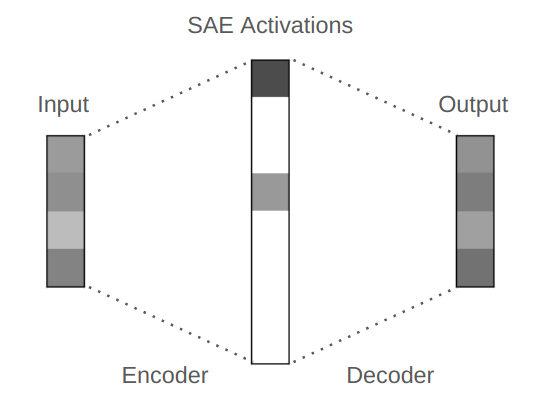
\includegraphics[width=0.84\textwidth,height=0.42\textheight,keepaspectratio]{SAE_diagram.png}
  \end{center}

  \vspace{0.22cm}
  {\centering\color{accent}\normalsize\textbf{This gives us a feature-level vocabulary for the residual stream}\par}
  \vspace{0.1cm}
  {\centering\color{muted}\scriptsize Building on Bricken et al. (2023) and Templeton et al. (2024)\par}
\end{frame}

% 7. Gap and RQ
\begin{frame}[plain]
  \vfill
  {\centering
    {\color{ink}\fontsize{23}{27}\selectfont\textbf{How do the features learned during pre-training change after post-training,}\par}
    \vspace{0.12cm}
    {\color{ink}\fontsize{23}{27}\selectfont\textbf{and how do they relate to behavioural changes?}\par}
  }
  \vfill
\end{frame}

% 8. Hypothesis
\begin{frame}{Hypothesis}
  \begin{beamercolorbox}[wd=\linewidth,sep=0.32cm,rounded=true]{normal text}
    {\Large\color{ink}\textbf{Empirical claim}}\\[0.2cm]
    {\normalsize\color{inktwo}
      Behaviorally central post-training features are mostly \textbf{modified} versions of pre-training features.
    }
  \end{beamercolorbox}
\end{frame}

% 9. Methodology
\begin{frame}{Methodology}{\textcolor{muted}{4 Stage Pipeline}}
  \begin{center}
    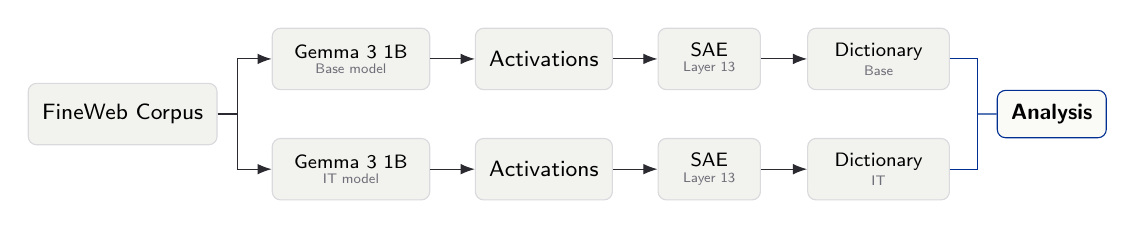
\begin{tikzpicture}[
      x=1cm, y=1cm,
      box/.style={draw=rule, fill=papersoft, rounded corners=3pt,
                  minimum height=0.78cm, align=center,
                  inner sep=5pt, font=\footnotesize},
      darrow/.style={-{Latex[length=1.8mm]}, color=inktwo},
    ]
      \node[box, minimum width=1.7cm] (fw) at (-3.7,0.75) {FineWeb Corpus};

      \node[box, minimum width=2.0cm] (m1) at (-0.8,1.45) {\shortstack[c]{\scriptsize Gemma 3 1B\\[-1pt]\textcolor{muted}{\fontsize{4.5pt}{5pt}\selectfont Base model}}};
      \node[box, minimum width=2.0cm] (m2) at (-0.8,0.05) {\shortstack[c]{\scriptsize Gemma 3 1B\\[-1pt]\textcolor{muted}{\fontsize{4.5pt}{5pt}\selectfont IT model}}};

      \node[box, minimum width=1.7cm] (a1) at (1.65,1.45) {Activations};
      \node[box, minimum width=1.3cm] (b1) at (3.75,1.45) {\shortstack[c]{\scriptsize SAE\\[-1pt]\textcolor{muted}{\fontsize{4.5pt}{5pt}\selectfont Layer 13}}};
      \node[box, minimum width=1.8cm] (c1) at (5.9,1.45) {\shortstack[c]{\scriptsize Dictionary\\[-1pt]\textcolor{muted}{\fontsize{4.5pt}{5pt}\selectfont Base}}};

      \node[box, minimum width=1.7cm] (a2) at (1.65,0.05) {Activations};
      \node[box, minimum width=1.3cm] (b2) at (3.75,0.05) {\shortstack[c]{\scriptsize SAE\\[-1pt]\textcolor{muted}{\fontsize{4.5pt}{5pt}\selectfont Layer 13}}};
      \node[box, minimum width=1.8cm] (c2) at (5.9,0.05) {\shortstack[c]{\scriptsize Dictionary\\[-1pt]\textcolor{muted}{\fontsize{4.5pt}{5pt}\selectfont IT}}};

      \node[draw=accent, fill=paper, rounded corners=3pt,
            inner sep=5pt, font=\footnotesize] (joint) at (8.1,0.75) {
        \textbf{Analysis}
      };
      \coordinate (mergeTop) at ($(c1.east)+(0.35,0)$);
      \coordinate (mergeBot) at ($(c2.east)+(0.35,0)$);
      \coordinate (mergeMid) at ($(mergeTop)!0.5!(mergeBot)$);

      \draw[darrow] (fw.east) -- ++(0.25,0) |- (m1.west);
      \draw[darrow] (fw.east) -- ++(0.25,0) |- (m2.west);
      \draw[darrow] (m1.east) -- (a1.west);
      \draw[darrow] (a1.east) -- (b1.west);
      \draw[darrow] (b1.east) -- (c1.west);
      \draw[darrow] (m2.east) -- (a2.west);
      \draw[darrow] (a2.east) -- (b2.west);
      \draw[darrow] (b2.east) -- (c2.west);

      \draw[-,color=accent] (c1.east) -- (mergeTop);
      \draw[-,color=accent] (c2.east) -- (mergeBot);
      \draw[-,color=accent] (mergeTop) -- (mergeBot);
      \draw[-,color=accent] (mergeMid) -- (joint.west);
    \end{tikzpicture}
  \end{center}
\end{frame}

% 10. Methodology analysis
\begin{frame}{Methodology}{\textcolor{muted}{Analysis}}
  \vspace{0.1cm}
  \begin{center}
    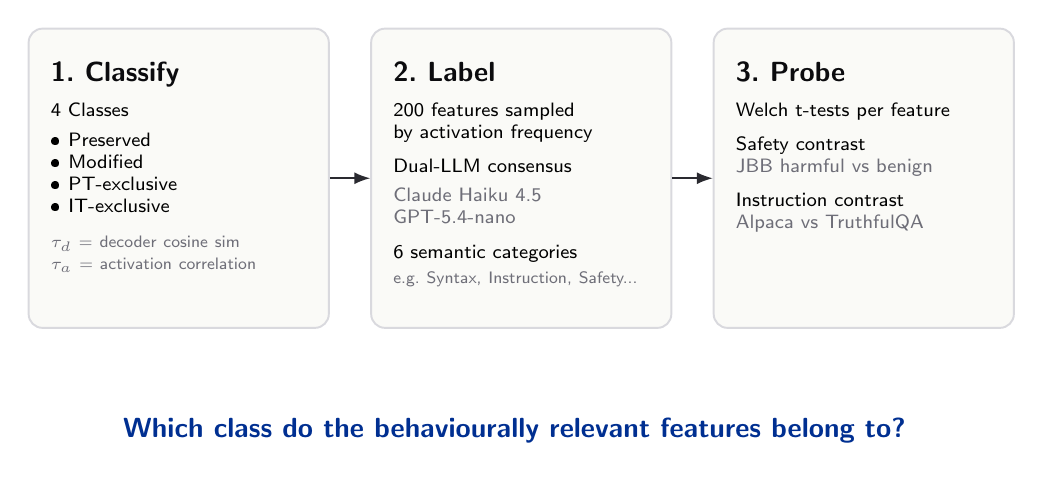
\begin{tikzpicture}[
      x=1cm, y=1cm,
      stepbox/.style={draw=rule, line width=0.7pt, fill=paper,
                      rounded corners=5pt, minimum width=3.2cm,
                      minimum height=3.8cm, text width=2.7cm,
                      align=left, inner sep=8pt, font=\scriptsize},
      link/.style={-{Latex[length=2mm]}, line width=0.55pt, color=inktwo},
      guide/.style={-{Latex[length=1.6mm]}, dashed, color=muted},
    ]
      \node[stepbox, minimum width=3.8cm, text width=3.25cm] (classify) at (-4.35,0.65) {
        \begin{minipage}[t][2.95cm][t]{3.25cm}
          \raggedright
          {\color{ink}\normalsize\textbf{1. Classify}}\\[0.16cm]
          4 Classes\\[0.10cm]
          \textbullet\ Preserved\\
          \textbullet\ Modified\\
          \textbullet\ PT-exclusive\\
          \textbullet\ IT-exclusive\\[0.16cm]
          {\color{muted}\fontsize{6.2pt}{6.8pt}\selectfont \mbox{$\tau_d$ = decoder cosine sim}}\\
          {\color{muted}\fontsize{6.2pt}{6.8pt}\selectfont \mbox{$\tau_a$ = activation correlation}}
        \end{minipage}
      };

      \node[stepbox, minimum width=3.8cm, text width=3.25cm] (label) at (0,0.65) {
        \begin{minipage}[t][2.95cm][t]{3.25cm}
          \raggedright
          {\color{ink}\normalsize\textbf{2. Label}}\\[0.16cm]
          200 features sampled\\
          by activation frequency\\[0.16cm]
          Dual-LLM consensus\\[0.08cm]
          {\color{muted}Claude Haiku 4.5}\\
          {\color{muted}GPT-5.4-nano}\\[0.16cm]
          6 semantic categories\\[0.04cm]
          {\color{muted}\fontsize{5.8pt}{6.4pt}\selectfont
          e.g.\ Syntax, Instruction, Safety...}
        \end{minipage}
      };

      \node[stepbox, minimum width=3.8cm, text width=3.25cm] (probe) at (4.35,0.65) {
        \begin{minipage}[t][2.95cm][t]{3.25cm}
          \raggedright
          {\color{ink}\normalsize\textbf{3. Probe}}\\[0.16cm]
          Welch t-tests per feature\\[0.16cm]
          Safety contrast\\
          {\color{muted}JBB harmful vs benign}\\[0.14cm]
          Instruction contrast\\
          {\color{muted}Alpaca vs TruthfulQA}
        \end{minipage}
      };

      \draw[link] (classify.east) -- (label.west);
      \draw[link] (label.east) -- (probe.west);

      \node[align=center, text=accent, font=\normalsize\bfseries] (question) at (0,-2.55) {
        Which class do the behaviourally relevant features belong to?
      };

    \end{tikzpicture}
  \end{center}
\end{frame}

% 10. Results
\begin{frame}{Results}{\textcolor{muted}{Modified Features Lead}}
  \vspace{0.40cm}
  \begin{center}
    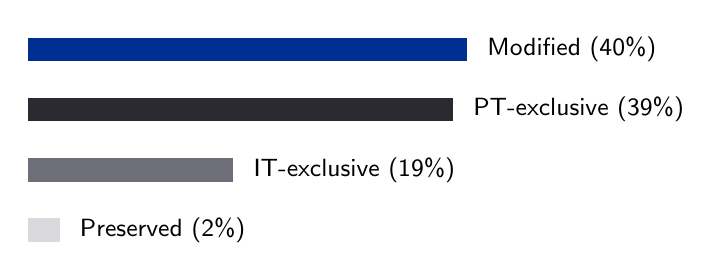
\begin{tikzpicture}[x=0.9cm,y=0.85cm]
      \fill[accent] (0,2.7) rectangle (6.2,3.05);
      \node[anchor=west] at (6.35,2.875) {\small Modified (40\%)};
      \fill[inktwo] (0,1.8) rectangle (6.0,2.15);
      \node[anchor=west] at (6.15,1.975) {\small PT-exclusive (39\%)};
      \fill[muted] (0,0.9) rectangle (2.9,1.25);
      \node[anchor=west] at (3.05,1.075) {\small IT-exclusive (19\%)};
      \fill[rule] (0,0) rectangle (0.45,0.35);
      \node[anchor=west] at (0.6,0.175) {\small Preserved (2\%)};
    \end{tikzpicture}
  \end{center}

  \vfill

  \begin{beamercolorbox}[wd=\linewidth,sep=0.24cm,rounded=true]{normal text}
    {\centering\normalsize\color{accent}\textbf{Post-training mostly reshapes pre-training features}\par}
  \end{beamercolorbox}
\end{frame}

% 11. Results (instruction contrast)
\begin{frame}{Results}{\textcolor{muted}{Did IT Create New Instruction Features?}}
  \vfill

  {\centering
    {\fontsize{38}{42}\selectfont\color{accent}\textbf{Mostly no}}\par
  }

  \vspace{0.65cm}

  \begin{columns}[c,totalwidth=\textwidth]
    \column{0.34\textwidth}
    \centering
    {\fontsize{30}{34}\selectfont\bfseries 19/20}\\[0.10cm]
    {\small\color{muted}instruction-style}\\[0.14cm]
    {\scriptsize\color{muted}%
      Top-ranked IT features on the\\[-0.05cm]
      Alpaca vs.\ TruthfulQA contrast}

    \column{0.32\textwidth}
    \centering
    {\fontsize{30}{34}\selectfont\bfseries 2/5}\\[0.10cm]
    {\small\color{muted}PT top-5 overlap}\\[0.14cm]
    {\scriptsize\color{muted}%
      Same indices in IT and PT\\[-0.05cm]
      top-5 under that contrast}

    \column{0.34\textwidth}
    \centering
    \chip{2006}\ \chip{446}\\[0.10cm]
    {\small\color{muted}\(+114.3\), \(+37.5\) in PT}\\[0.14cm]
    {\scriptsize\color{muted}%
      Example shared features;\\[-0.05cm]
      per-prompt activation deltas}
  \end{columns}

  \vfill

  {\centering\normalsize\color{inktwo}\textbf{Shared} and \textbf{modified}, not IT-exclusive.\par}

  \vspace{0.35cm}
\end{frame}

% 12. Main takeaway
\begin{frame}{Main takeaway}
  \begin{beamercolorbox}[wd=\linewidth,sep=0.3cm,rounded=true]{normal text}
    {\normalsize\color{inktwo}Post-training appears to mainly \textbf{reorganize, amplify, and sharpen existing pre-training features}, rather than creating entirely new internal structure.}
  \end{beamercolorbox}

  \vspace{0.2cm}

  \begin{beamercolorbox}[wd=\linewidth,sep=0.3cm]{normal text}
    {\normalsize\color{inktwo}The evidence therefore supports a \textbf{weak but consistent claim}:}
    \begin{itemize}
      \item Behaviorally central post-training features are usually transformed versions of pre-training features.
    \end{itemize}
  \end{beamercolorbox}
\end{frame}

% 14. Limitations & next steps
\begin{frame}{Limitations \& Next Steps}
  \vspace{0.15cm}
  \begin{columns}[T,totalwidth=\textwidth]
    \column{0.31\textwidth}
    \begin{minipage}[t][2.6cm][t]{\linewidth}
      {\large\color{ink}\textbf{Correlational evidence}}\\[0.12cm]
      {\color{muted}\rule{\linewidth}{0.35pt}}\\[0.12cm]
      {\scriptsize\color{inktwo}The analysis links feature shifts to behavior, but does not yet prove causal effects.}
    \end{minipage}

    \vspace{0.18cm}
    {\scriptsize\color{accent}\textbf{Next:} Test whether steering high-impact modified features affects model behavior.}

    \column{0.31\textwidth}
    \begin{minipage}[t][2.6cm][t]{\linewidth}
      {\large\color{ink}\textbf{Imperfect labeling}}\\[0.12cm]
      {\color{muted}\rule{\linewidth}{0.35pt}}\\[0.12cm]
      {\scriptsize\color{inktwo}Labels are partly interpretive; inter-annotator agreement reached about 60\%.}
    \end{minipage}

    \vspace{0.18cm}
    {\scriptsize\color{accent}\textbf{Next:} Refine the labeling strategy.}

    \column{0.31\textwidth}
    \begin{minipage}[t][2.6cm][t]{\linewidth}
      {\large\color{ink}\textbf{Narrow scope}}\\[0.12cm]
      {\color{muted}\rule{\linewidth}{0.35pt}}\\[0.12cm]
      {\scriptsize\color{inktwo}One model family, one architecture size, and one layer only.}
    \end{minipage}

    \vspace{0.18cm}
    {\scriptsize\color{accent}\textbf{Next:} Replicate the pipeline across more layers, model sizes, and model families.}
  \end{columns}
\end{frame}

% 15. Why this matters
\begin{frame}{Why this matters}
  \vspace{0.1cm}
  \begin{columns}[T,totalwidth=\textwidth]
    \column{0.48\textwidth}
    \begin{minipage}[t][3.45cm][t]{\linewidth}
      {\large\color{ink}\textbf{Behavior is not representation}}\\[0.14cm]
      {\color{muted}\rule{\linewidth}{0.35pt}}\\[0.14cm]
      {\small\color{inktwo}
      Benchmarks measure outputs.\\[0.08cm]
      They do not reveal internal structure.\\[0.08cm]
      Safety still rests on fragile representations.}
    \end{minipage}

    \column{0.48\textwidth}
    \begin{minipage}[t][3.45cm][t]{\linewidth}
      {\large\color{ink}\textbf{Interpretability must catch up}}\\[0.14cm]
      {\color{muted}\rule{\linewidth}{0.35pt}}\\[0.14cm]
      {\small\color{inktwo}
      Deployment is ahead of understanding.\\[0.08cm]
      SAEs are starting to close that gap.\\[0.08cm]
      The real test is applying them to deployed frontier models.}
    \end{minipage}
  \end{columns}

  \vfill

  \begin{beamercolorbox}[wd=\linewidth,sep=0.26cm,rounded=true]{normal text}
    {\centering\normalsize\color{accent}\textbf{This is an important and necessary step towards safer,\\ more reliable and aligned models}\par}
  \end{beamercolorbox}
\end{frame}

\begin{frame}[plain]
  \vfill
  \begin{center}
    {\color{ink}\Huge\textbf{Questions}}
  \end{center}
  \vfill
\end{frame}

\end{document}
